\graphicspath{ {Figures/Pileup/Multiplier/} {Figures/Pileup/Phase/} {Figures/Pileup/EnergyScaling/} {Figures/RandomSeeds/FitStartScans/} {Figures/RandomSeeds/FitIterations/} {Figures/Miscellaneous/} {Figures/FitStartScans/} {Figures/CBO/Frequency/} {Figures/CBO/Shape/} {Figures/CBO/LifetimeScan/} {Figures/Gain/InFill/} {Figures/VW/} {Figures/LostMuons/} }

\chapter{Systematic Uncertainty Evaluations}
\label{Ch:Systematics}

\section{Sensitivity of \texorpdfstring{$\omega_{a}$}{} to gain corrections}
\label{Sec:SystematicGain}

	I estimate the systematic error on R due to the the in-fill gain function at 24.8 ppb, and to the Short Term Double Pulse correction at blank ppb. Adding these in quadrature results in a systematic error of blank ppb.

	\subsection{In-Fill Gain}

		As positrons hit the calorimeters throughout the fill, there will be a gain sag response such that the energy of detected positrons changes throughout the fill, dropping at first and then rising exponentially back up to their true values. This changing energy response will lead to a systematic error on R, as positrons with mis-measured energies near the energy threshold are excluded from the fit. This gain sag is corrected for in the Recon West code, before I fill my histograms. Due to the way I've constructed my analysis code, it's not so simple to modify the reconstruction code and create new histograms quickly. Such a process would require the rebuilding of many sets of new cluster root trees, and then making histograms from those. As a faster way of getting at the in fill gain systematic error, I've instead chosen to apply a gain sag function to the incoming energy-corrected clusters. This allows me to scan over gain sag function parameters and only run off one set of trees, as I've been doing for all systematic studies.

		(Should this bit be in the analysis procedures chapter?) The in-fill gain sag function was determined by Matthias Smith and the laser team as shown in \DB{14077}. (Cite or link?) The function goes as  
			\begin{gather}
				E = E_{0}(1 - A \cdot e^{-(t-t_{offset})/\tau}),
			\label{Eqn:GainSag}
			\end{gather}
		where $E_{0}$ is the orginal energy of the positron cluster, A is the amplitude factor on the gain sag function, $\tau$ the lifetime, and then $t_{offset}$ the shift of the function from 0. It is this function that is inverted and applied to the clusters in the reconstruction. I apply a function of the same form in my own code before filling hits into histograms, in essence undoing the reconstruction gain correction as a way to measure the in-fill gain sag effect on R.

		\begin{figure}[h]
			\centering
			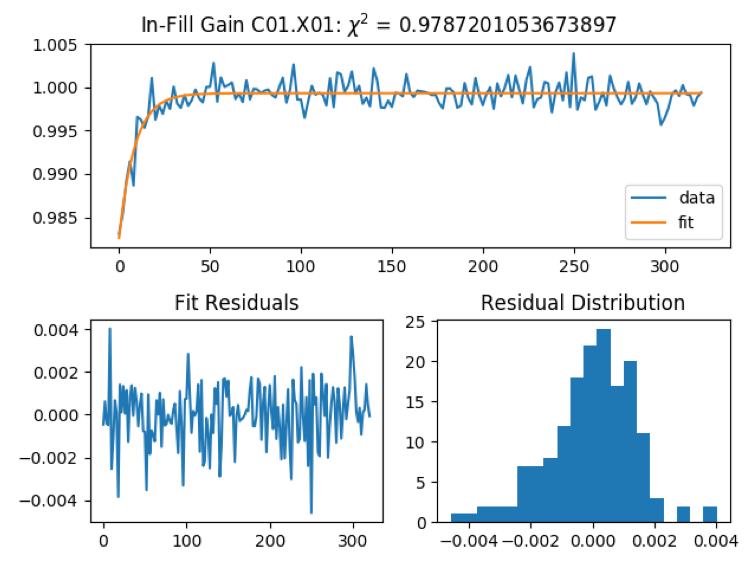
\includegraphics[width=.8\textwidth]{MatthiasInFill}
		    \caption[MatthiasInFill]{The top plot shows the in-fill gain sag function in orange from a fit to data in blue, for crystal 1 in calorimeter 1. The gain sag can be modeled effectively by a simple exponential function. By $\SI{30}{\mu s}$ the change in energy response is nearly only .1\%. (Might want to look up these exact numbers.) The bottom two plots show the residuals of the fit. Plot made by Matthias Smith.}
		    \label{Fig:MatthiasInFill}
		\end{figure}

		There are some simplifications and assumptions I've made when applying said gain sag function in my own code. First is that while in the reconstruction code each crystal of each calorimeter has its own singular in-fill gain function, one of which is shown in Figure \ref{Fig:MatthiasInFill}, I apply a global gain sag function to all incoming clusters. Secondly the default parameters for the gain sag function are simply eyeballed from the fcl file where all crystal parameters are stored. These values are 0.03 for the amplitude, $\SI{6.7}{\mu s}$ for the lifetime, and $\SI{3.907}{\mu s}$ for the offset. (Once the latest dataset is available I will need to come up with a better way to apply this gain sag function, either with multiple functions per crystal or with parameters that are actual averages. For now it's fine though to get words on the paper.) Finally, I apply this gain sag function after I apply the artificial deadtime to the incoming clusters, due to code restrictions. This should be a small effect. These assumptions I believe should be okay as long as I take my systematic errors conservatively.

		\begin{figure}[]
		\centering
		    \begin{subfigure}[t]{0.45\textwidth}
			    \centering
				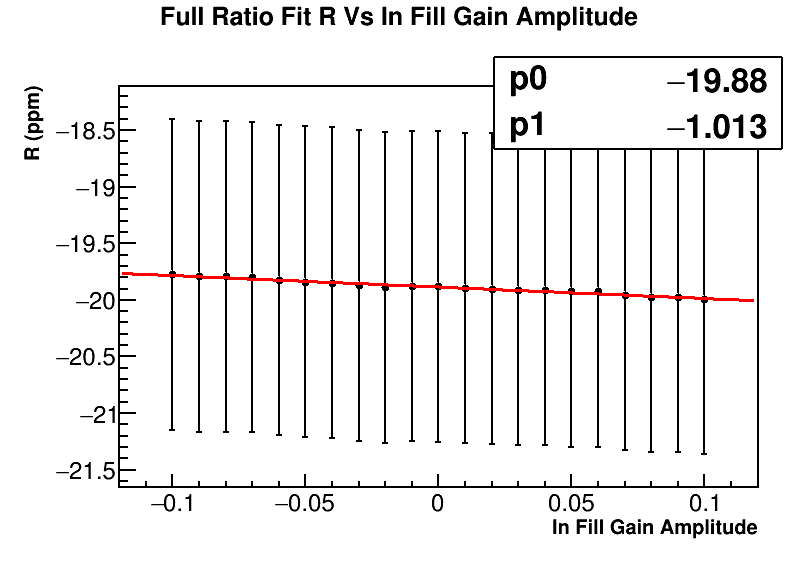
\includegraphics[width=\textwidth]{RatioCBO_R_Vs_InFillGainAmplitude_Canv}
			    \caption{Plotted is R vs the amplitude parameter in the gain sag function. The slope is -1.013 ppm per unit amplitude.}
		    \end{subfigure}
		    \hspace{4mm}
		    \begin{subfigure}[t]{0.45\textwidth}
			    \centering
				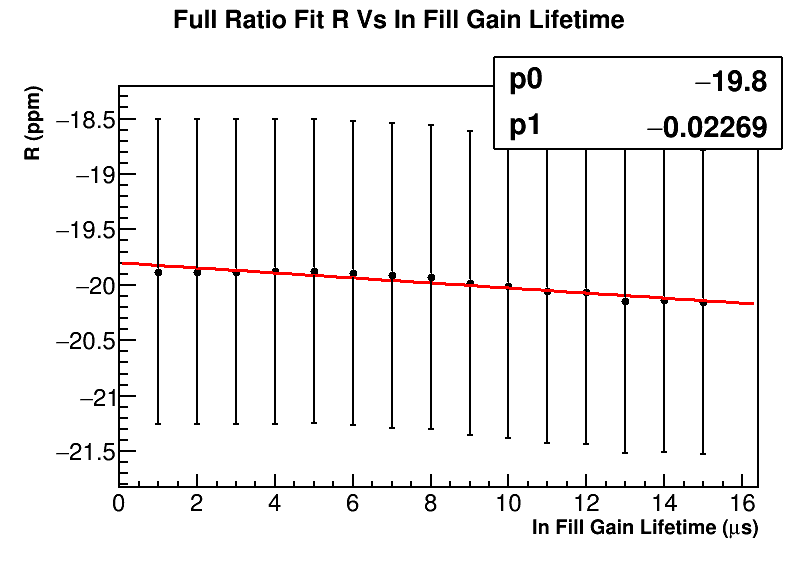
\includegraphics[width=\textwidth]{RatioCBO_R_Vs_InFillGainLifetime_Canv}
			    \caption{Plotted is R vs the lifetime parameter in the gain sag function. The slope is -0.02269 ppm per $\mu s$.}
		    \end{subfigure}% %you need this % here to add spacing between subfigures
		    \vspace{4mm}
		    \begin{subfigure}[t]{0.45\textwidth}
			    \centering
				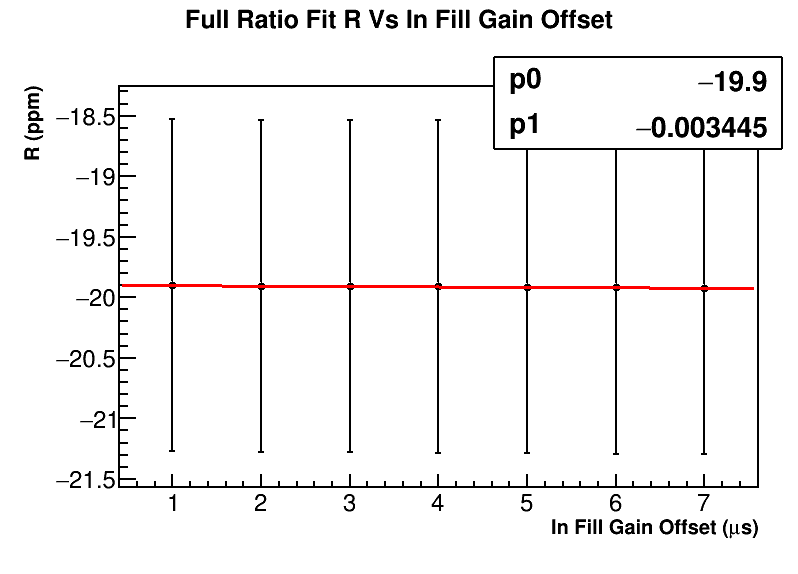
\includegraphics[width=\textwidth]{RatioCBO_R_Vs_InFillGainOffset_Canv}
			    \caption{Plotted is R vs the offset parameter in the gain sag function. The slope is -0.0034 ppm per $\mu s$.}
		    \end{subfigure}% %you need this % here to add spacing between subfigures
		\caption[InFillGain]{Plotted is fitted R values vs gain sag function parameters. In each case I scanned over ranges approximately centered around the eyeballed average values.}
		\label{Fig:InFillGain}
		\end{figure}

		To calculate the systematic error, I simply scan over the gain sag function parameters and observe the changes in R. This includes scans over the amplitude, lifetime, and offset as described in \ref{Eqn:GainSag}, and shown in Figure \ref{Fig:InFillGain}. I calculate the systematic error on R as the quadrature sum of the separate pieces as 
		\begin{align}
			\delta R_{A} &= \delta\alpha_{A} \times \frac{dR}{d\alpha_{A}}, \\
			\delta R_{\tau} &= \delta\alpha_{\tau} \times \frac{dR}{d\alpha_{\tau}}, \\
			\delta R_{offset} &= \delta\alpha_{offset} \times \frac{dR}{d\alpha_{offset}},
		\end{align}
		where $\delta\alpha_{A}$, $\delta\alpha_{\tau}$, and $\delta\alpha_{offset}$ are the uncertainties on the gain sag amplitude, lifetime, and offset respectively. I take the uncertainty on the amplitude very conservatively at 1\%, leading to a systematic error on R of $0.01 \times \SI{1.013}{ppm} = \SI{10.1}{ppb}$. I take the uncertainty on the lifetime very conservatively at $\SI{1}{\mu s}$, leading to a systematic error on R of $1 \times \SI{22.7}{ppb} = \SI{22.7}{ppb}$. Finally the slope for the offset parameter is very flat, and that combined with a very uniform array of values for the offset parameter in the reconstruction (indicative of a very small uncertainty), means that the systematic error on R is negligible. Therefore I ignore the offset parameter and add the amplitude and lifetime errors in quadrature to produce a systematic error on R of 24.8 ppb. (The uncertainty on the parameters would be the fit errors on the parameter I think, except for the fact that I'm using a global gain sag function as opposed to crystal functions, meaning the uncertainty might be the spread in parameters. I'm not entirely sure. Also I have removed the offset parameter in my latest code and will reproduce these results without it with the new dataset when it's available.)

	\subsection{Short Term Double Pulse (SDTP)}

		Work and writing to be done here. I plan on reconstructing clusters w/ and w/o the SDTP included and comparing the results to determine the systematic effect on R.


\section{Sensitivity of \texorpdfstring{$\omega_{a}$}{} to pileup}
\label{Sec:SystematicPileup}

	The systematic error on R due to the pileup construction consists primarily of two parts, the error due to misconstruction of the amplitude and the phase of the pileup. I estimate the systematic error on R due to the pileup amplitude at 22.6 ppb, and to the pileup phase in pieces of 25.7 and 16.1 ppb. Adding these in quadrature results in a systematic error of 37.8 ppb.

	\subsection{Pileup Amplitude}

		The error due to the amplitude misconstruction was calculated by scanning over a pileup multiplier parameter, from 90\% of the calculated pileup amplitude to 110\%, as shown in Figure \ref{fig:PileupMultiplier}. The sensitivity of R to the amplitude was determined to be -509.1 ppb per unit amplitude. The uncertainty of the pileup amplitude construction was determined by fitting a parabola to the \chisq as a function of the pileup amplitude, and taking the width of that parabola as the uncertainty. This width is determined as the distance in X for the \chisq to rise by 1 from the minimum, also calculated as $\sqrt{2/(\chi^{2})''}$.

		\begin{figure}[h]
		\centering
		    \begin{subfigure}[t]{0.45\textwidth}
			    \centering
				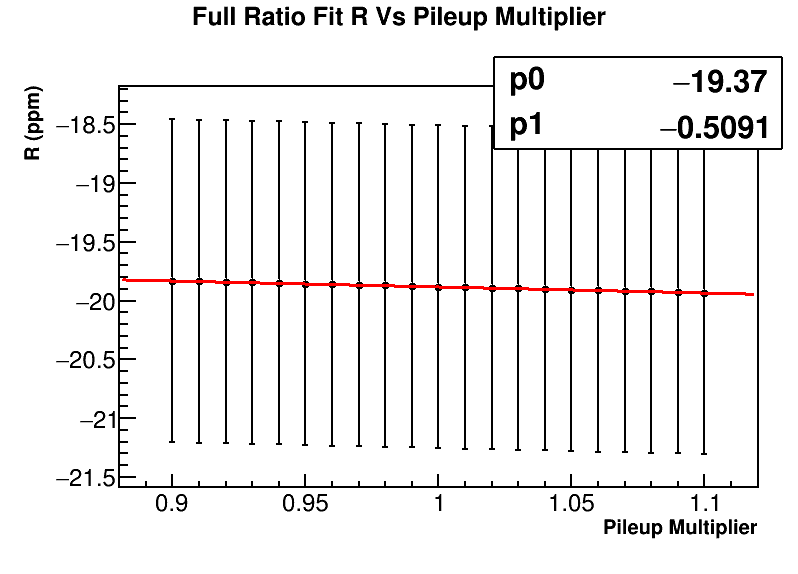
\includegraphics[width=\textwidth]{RatioCBO_R_Vs_PileupMultiplier_Canv}
			    \caption{Sensitivity of R vs the pileup amplitude. The slope is -509.1 ppb per unit amplitude.}
		    \end{subfigure}
		    \hspace{4mm}
		    \begin{subfigure}[t]{0.45\textwidth}
			    \centering
				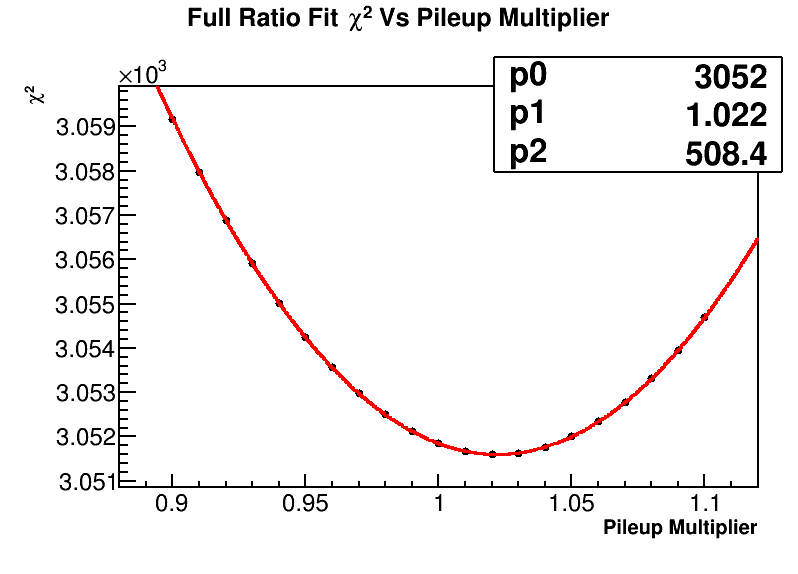
\includegraphics[width=\textwidth]{RatioCBO_Chi2_Vs_PileupMultiplier_Canv}
			    \caption{Plotted is the fitted \chisq vs the pileup amplitude. The fit equation used was $p2 \times (x - p1)^{2} + p0.$ The minimum lies at 1.022.}
		    \end{subfigure}
		\caption[PileupMultiplier]{The significant plots to determine the pileup amplitude systematic error.}
		\label{fig:PileupMultiplier}
		\end{figure}

		This corresponds to an uncertainty of $\sqrt{1/508.4} = 0.0444$ or 4.44\%. The minimum of the \chisq plot of 1.022 lies at approximately .5$\sigma$ away from 1, which is consistent and nice to see. Then, calculating the systematic error on R due to the pileup amplitude construction as 
			\begin{align}
				\delta R_{pm} = \delta\alpha_{pm} \times \frac{dR}{d\alpha_{pm}}
			\end{align}
		where $\delta\alpha_{pm}$ is the uncertainty on the pileup amplitude, the systematic error on R is calculated as $0.0444 \times \SI{509.1}{ppb} = \SI{22.6}{ppb}$.

		Another technique to estimate the uncertainty of the pileup amplitude construction is to look at the offset of the high energy tail of the pileup subtracted energy spectrum from zero. Because however I've applied only the doublet correction, I know that the shape of the pileup spectrum is wrong by some amount, as evidenced in Figure \ref{fig:AddedEnergies}. While the pileup itself can multiplied by some scaling factor other than 1 in order to align the energy spectra slightly better, because the shape of the pileup correction is imperfect the offset calculation I believe is the wrong way to go about calculating this uncertainty in my case. The shape can be fixed by including the triplets and the doublet contamination in the shadow method, but that work is incomplete. Since the triplets are a 1\% effect relative to the doublets, and the contamination is of the same order, I believe the uncertainty of 4.44\% conservatively includes for this mismatch in shape and the omission of the triplets. Regardless, since the statistics of the 60H dataset is much larger than the order of the systematic effect for the pileup construction ($\mathcal{O}$(1 ppm) vs $\mathcal{O}$(10 ppb)), this is a fine assumption.

	\subsection{Pileup Phase}
	\label{SubSec:PileupPhase}

		The error on R due to the pileup phase construction was calculated by scanning over a pileup time shift parameter, where the pileup spectrum was shifted in time by some amount before subtraction. The sensitivity of R to this parameter is shown in Figure \ref{fig:PileupPhase}. It is extremely unlikely that the entire pileup spectrum could be shifted by the offsets shown here, so this is a conservative estimate of the effect of the pileup phase on R. I then calculate the phase error as 
			\begin{align}
				\delta R_{pp} = \delta\alpha_{pp} \times \frac{dR}{d\alpha_{pp}}
			\end{align}
		where $\delta\alpha_{pp}$ is the uncertainty on the pileup phase. Conservatively estimating the uncertainty on the pileup phase as half the artificial deadtime at 3 ns, the systematic error on R is then calculated as $\SI{3}{ns} \times \SI{8.571}{ppb/ns} = \SI{25.7}{ppb}$. Figure \ref{fig:PileupTimeShiftFS} shows the change in R vs fit start times for pileup time shifted spectra vs the unshifted pileup time spectra. As shown the difference converges to zero as the level of pileup diminishes over the course of a fill.

		\begin{figure}[]
			\centering
			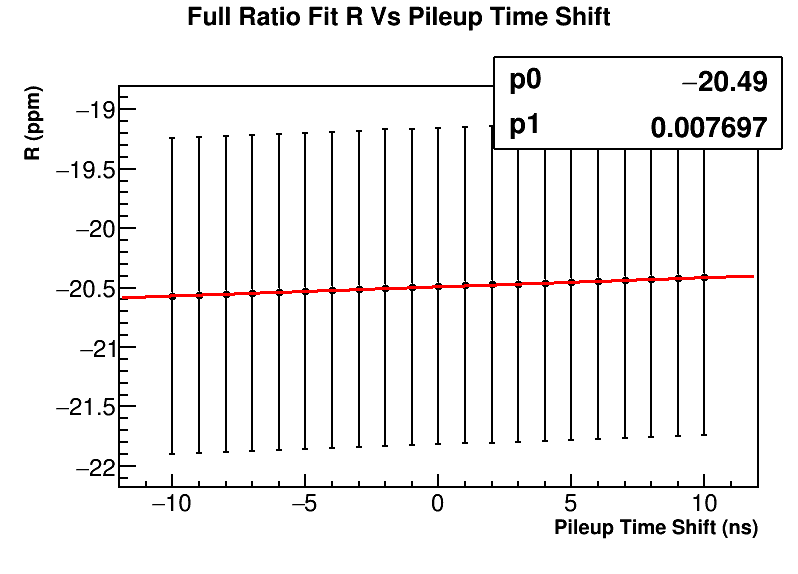
\includegraphics[width=.5\textwidth]{RatioCBO_R_Vs_PileupTimeShift_Canv}
		    \caption[PileupPhase]{Sensitivity of R vs the pileup phase. The slope is 8.571 ppb per ns.}
		    \label{fig:PileupPhase}
		\end{figure}

		\begin{figure}[]
			\centering
			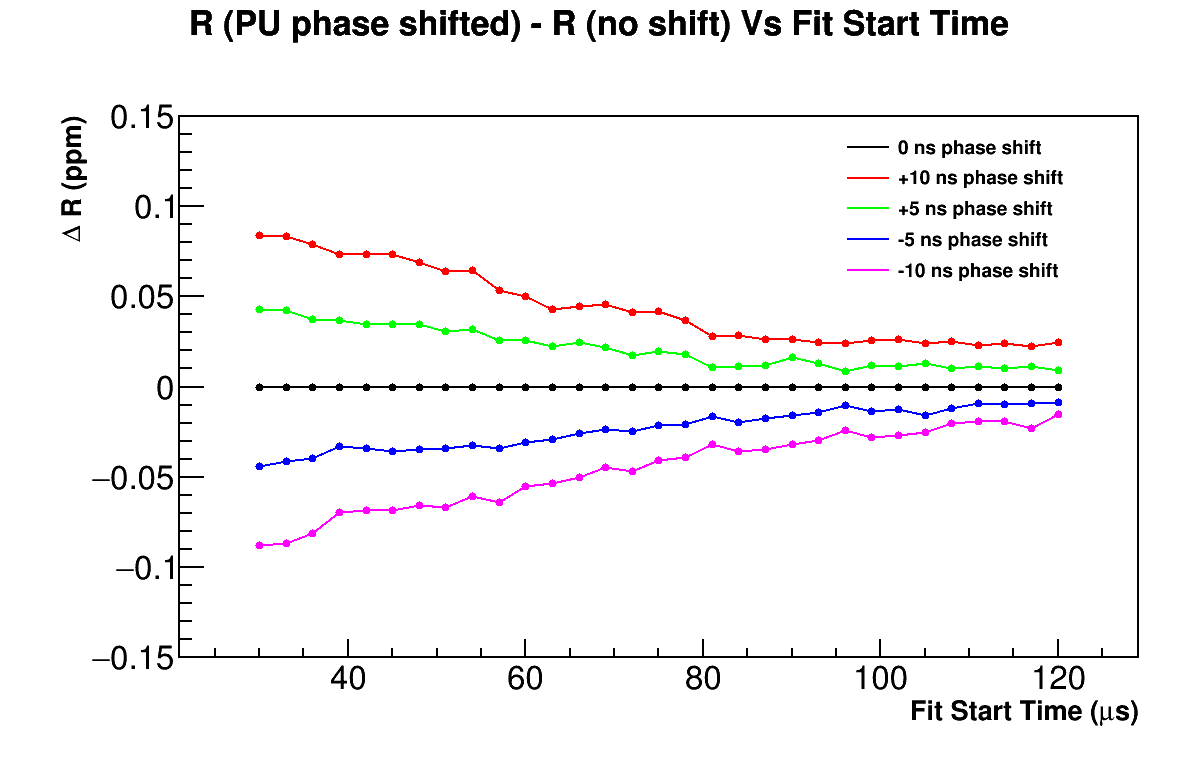
\includegraphics[width=.8\textwidth]{pileupTimeShiftComparison}
		    \caption[PileupTimeShiftFS]{Plotted is $\Delta R$ between pileup time shifted and unshifted results vs fit start time. The black line and points are by definition 0. As the fit start time increases and the pileup reduces, the $\Delta R$ points converge to zero as they should.}
		    \label{fig:PileupTimeShiftFS}
		\end{figure}

		As mentioned in section Section \ref{Sec:PileupCorrection}, the energy of the pileup pulses may not actually be exactly equal to the sum of the pileup singlets. If the energy of the pileup pulses are systematically miscalculated, then doublets will be added or lost near the energy threshold applied when constructing the pileup spectrum. This leads to an additional error on the phase which needs to be included. With the energy of the pileup pulses calculated as
			\begin{align}
				E_{doublet} = C \cdot (E_{1} + E_{2}),
			\end{align}
		by scanning over the parameter C this error can be determined. The sensitivity of R to this pileup energy scaling parameter is shown in Figure \ref{fig:PileupEnergyScaling}, with a slope of -806.5 ppb per unit scaling parameter. The systematic error on R is calculated in the usual way,
			\begin{align}
				\delta R_{pe} = \delta\alpha_{pe} \times \frac{dR}{d\alpha_{pe}}
			\end{align}
		where $\delta\alpha_{pe}$ is the uncertainty on the pileup energy dependence. This uncertainty was calculated in the same manner as was done for the pileup amplitude, by fitting a parabola to the \chisq as a function of the energy scaling parameter, and it was determined to be 2\%. The systematic error on R is then calculated as $0.02 \times \SI{806.5}{ppb} = \SI{16.1}{ppb}$.

		\begin{figure}[]
		\centering
		    \begin{subfigure}[t]{0.45\textwidth}
			    \centering
				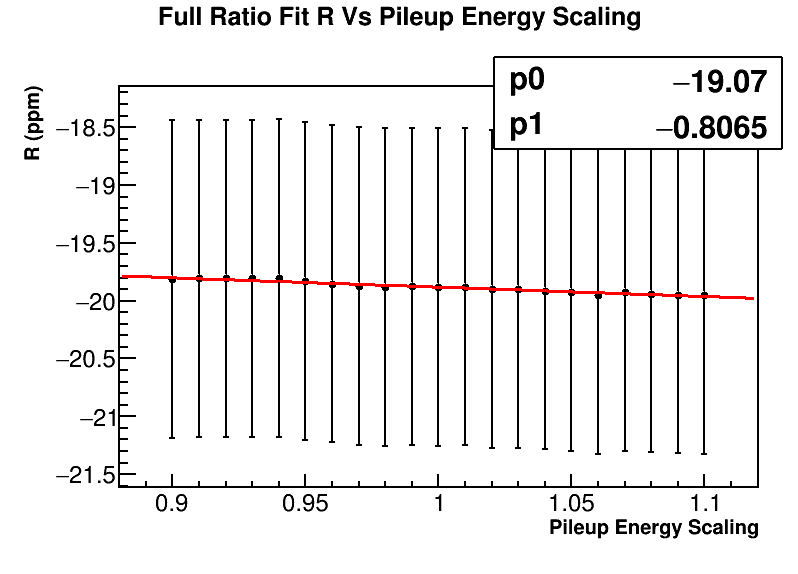
\includegraphics[width=\textwidth]{RatioCBO_R_Vs_PileupEnergyScaling_Canv}
			    \caption{Sensitivity of R vs the pileup energy scaling parameter. The slope is -806.5 ppb per unit energy scaling.}
		    \end{subfigure}
		    \hspace{4mm}
		    \begin{subfigure}[t]{0.45\textwidth}
			    \centering
				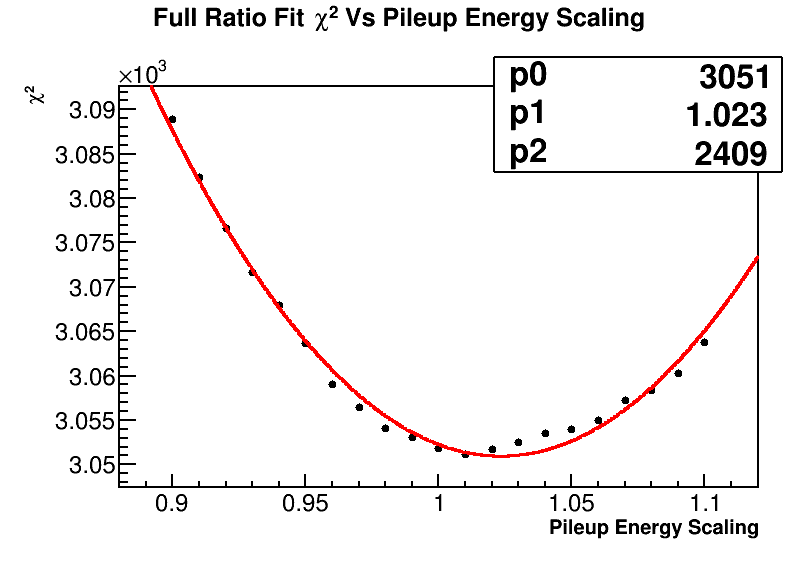
\includegraphics[width=\textwidth]{RatioCBO_Chi2_Vs_PileupEnergyScaling_Canv}
			    \caption{Plotted is the fitted \chisq vs the pileup energy scaling parameter. The fit equation used was $p2 \times (x - p1)^{2} + p0.$ The minimum lies at 1.023.}
		    \end{subfigure}
		\caption[PileupEnergyScaling]{The significant plots to determine a part of the pileup phase systematic error.}
		\label{fig:PileupEnergyScaling}
		\end{figure}


\section{Sensitivity of \texorpdfstring{$\omega_{a}$}{} to lost muons}
\label{Sec:SystematicLM}

	I estimate the systematic error on R due to the lost muon function at 36.1 ppb, and to the lost muon bias as

	\subsection{Lost muon function}

		As described in Section \ref{Sec:LM}, the lost muon function does not need to be included in the ratio fit. In order to calculate a systematic error from excluding the lost muon function, I added the function to the fit as described in that section. I fixed the value of the $\kappa_{loss}$ parameter to that determined from a T Method fit of the same data. The results can be seen in Figure \ref{fig:LMModuloPlot}. The final fitted R value differs from the non-LM fitted function by -36.1 ppb. Therefore I take the the systematic error from excluding the lost muon function as 36.1 ppb. 

		\begin{figure}[]
			\centering
			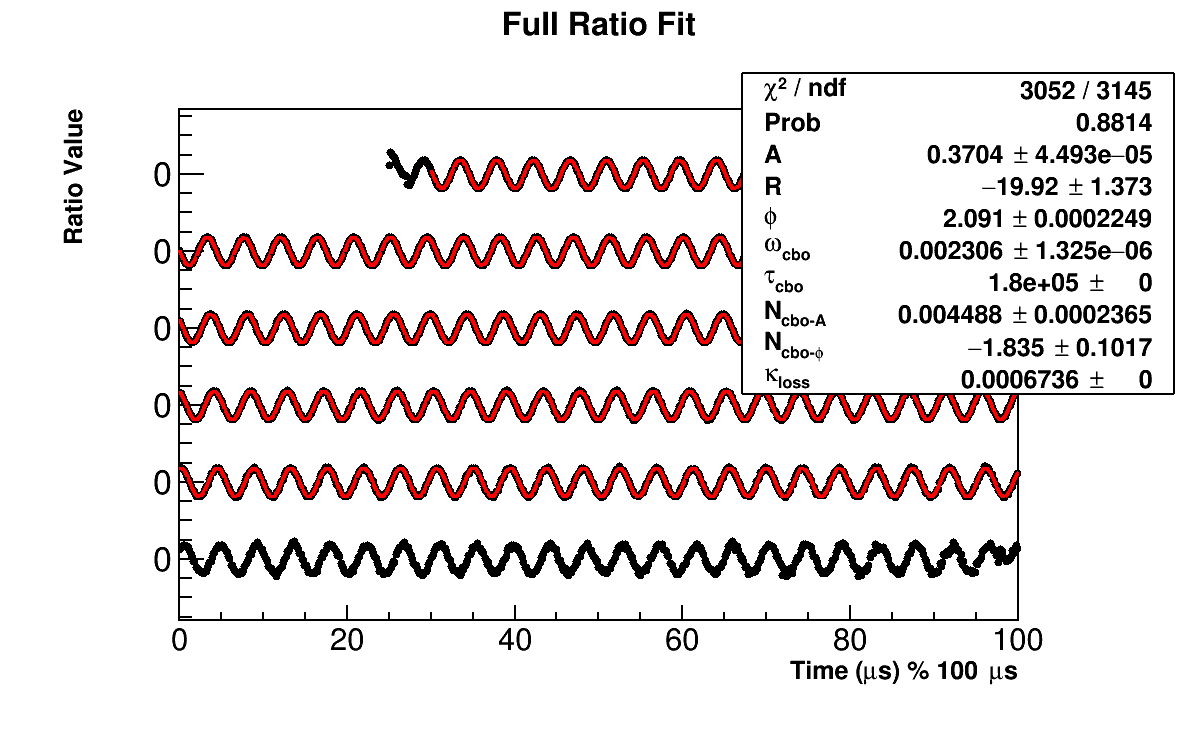
\includegraphics[width=\textwidth]{ratioCBO_moduloPlot-lostmuonsfixed}
		    \caption[LMModuloPlot]{Fit results with the LM term included. The lost muon parameter has been fixed. The x axis is in units of $\mu$s modulo 100 $\mu$s, with successive portions of the data points and fit shifted downwards on the plot. The parameter values in the stats box for the CBO frequency and lifetime are in units of ns. R is blinded locally. The fit ranges from 30 $\mu$s to 500 $\mu$s.}
		    \label{fig:LMModuloPlot}
		\end{figure}


	\subsection{Lost muon bias}


\section{Sensitivity of \texorpdfstring{$\omega_{a}$}{} to CBO function}
\label{Sec:SystematicCBO}

	I estimate the systematic error on R due to the CBO frequency at 30 ppb, to the CBO envelope shape at 21.1 ppb, and to the fixed CBO lifetime at 12.1 ppb. Adding these in quadrature results in a systematic error of 38.6 ppb.

	\subsection{CBO Frequency}
	\label{Sec:CBOFreq}

	As described in Section \ref{Sec:CBO}, the CBO frequency as a function of time changes over the course of a fill. Shown in Figure \ref{fig:CBOFreqModel} is a comparison between the fitted CBO frequency parameter as a function of fit start time for a constant frequency vs a changing frequency. Without the changing frequency the fit behaves improperly. Because a specific model was chosen for the CBO frequency, there will be a systematic error on R that needs to be determined. James Mott examined the frequency function he derived from the data in greater detail in \DB{15376}, where he considered parameter correlations in Equation \ref{Eqn:CBOFreq} and subsequent effects on the overall function. He found that errors were small, parameters were highly correlated, and that the CBO frequency function was very well constrained, as well as comparable between stations 12 and 18, and the 60H and 9d datasets. 

	In order to determine the systematic error on R, I simply varied the individual fixed parameters in the CBO frequency function $\{\Delta\omega, A, \tau_{A}, B, \tau_{B}\}$, by $\pm 2 \sigma$, where the errors on the parameters were taken from \DB{15376}. I also fit the data with the station 18 parameters. Even though the frequency parameters are highly correlated, varying them individually should be a conservative method for determining the overall systematic error on R. I found a 25 ppb difference in the fitted R value for the station 18 parameters, as compared to the station 12 parameters, primarily due to the different ``A'' value, and differences of order 5 ppb or less for the rest of the parameters. Adding them in quadrature resulted in an error of approximately 27.3 ppb. In order to be slightly more conservative, I estimate the systematic error on R due to the frequency at 30 ppb.

		\begin{figure}[]
		\centering
		    \begin{subfigure}[t]{0.45\textwidth}
			    \centering
				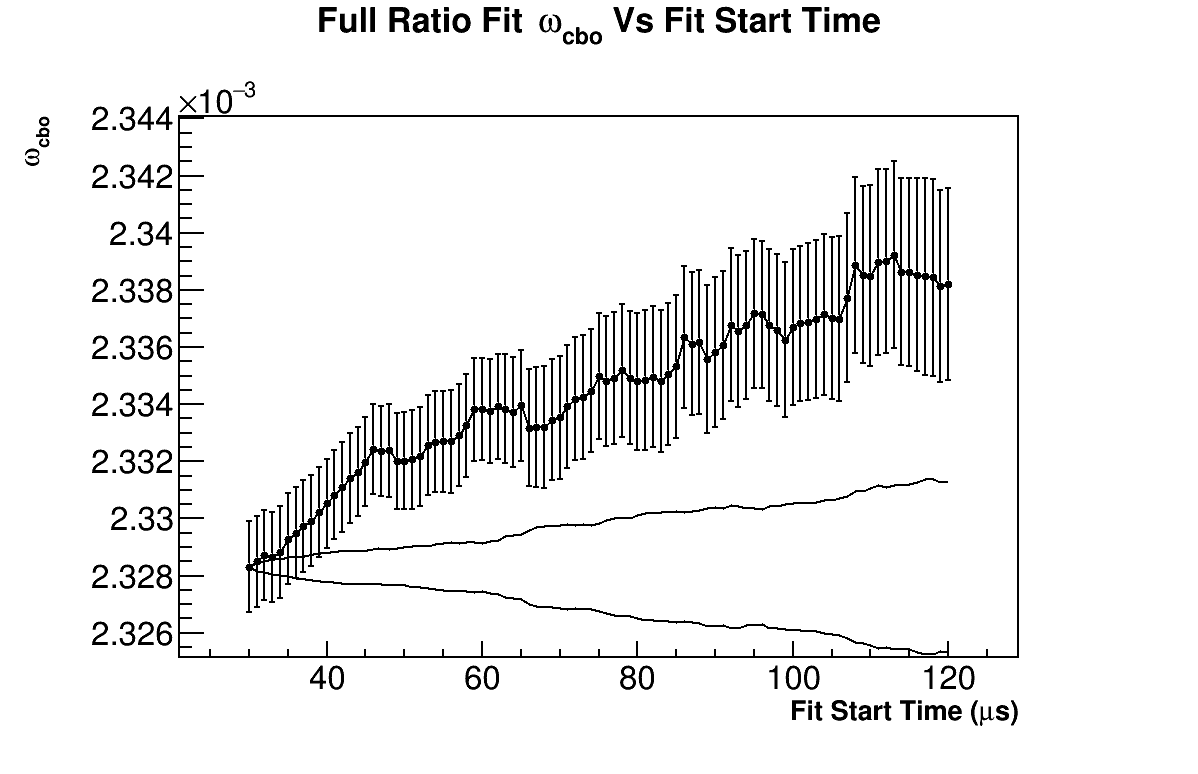
\includegraphics[width=\textwidth]{fixed-wcbo-vs-fs}
			    \caption{Fixed CBO frequency.}
		    \end{subfigure}
		    \hspace{4mm}
		    \begin{subfigure}[t]{0.45\textwidth}
			    \centering
				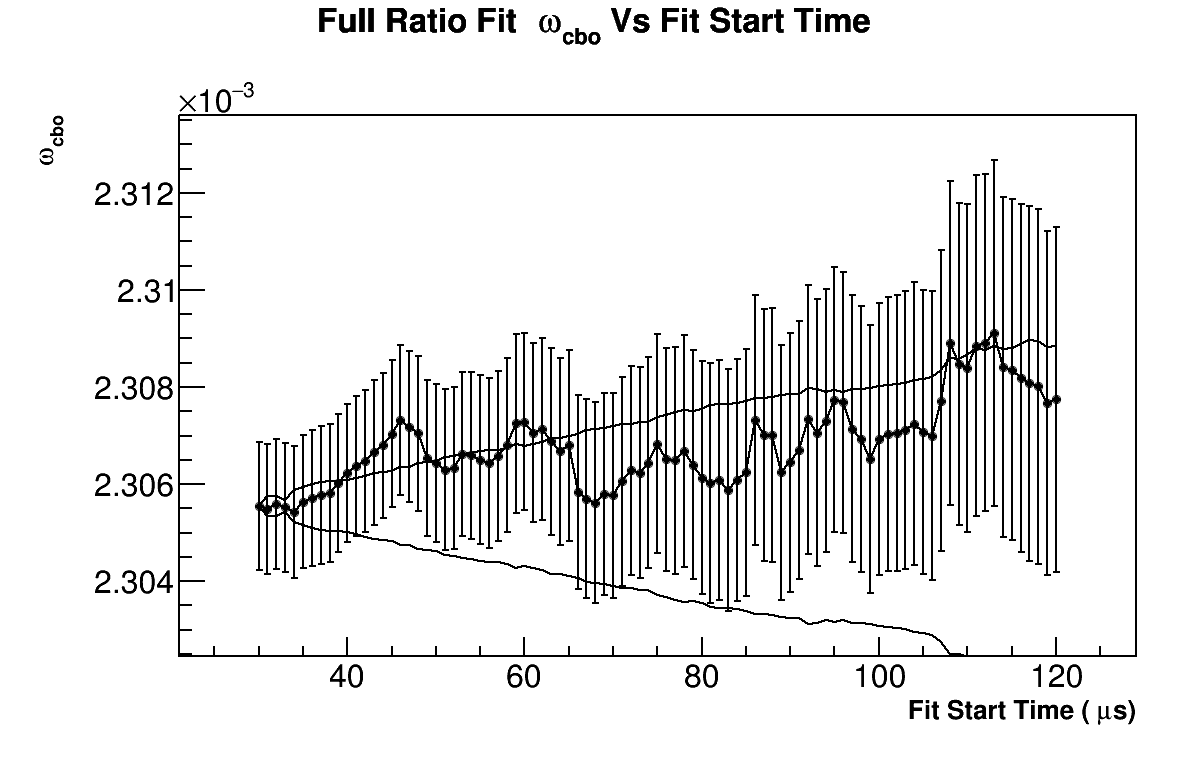
\includegraphics[width=\textwidth]{RatioCBO_omega_cbo_FS_Canv}
			    \caption{Changing CBO frequency.}
		    \end{subfigure}
		\caption[CBOFreqModel]{Fit start time scans for the CBO frequency parameter with a fixed frequency (left) and for the tracker model frequency (right). With the inclusion of the changing frequency over time, the fit parameter becomes stable as a function of fit start time.}
		\label{fig:CBOFreqModel}
		\end{figure}


	\subsection{CBO Shape}
	\label{SubSec:CBOShape}

		If the shape of the CBO in the fit function is wrong, then there will be a systematic error on R. Because I get good fits and the CBO parameters are stable vs fit start time, the possbile changes to the envelope are limited, compared to the envelope used as shown in Equation \ref{eqn:CBO}. Possible changes to the envelope include those functions as shown in Figure \ref{fig:CBOShapeAmplitude}, an exponential plus a constant and then an exponential times another oscillatory term. Both new envelopes were determined from tracker analysis fits to the CBO amplitude. Both changes to the envelope amplitude were tried in the fitting function, with changes in R of $\SI{-21.1}{ppb}$ and $\SI{-9.6}{ppb}$ respectively, though neither showed any improvement in the fit. (In the latter the period of the oscillatory term was fixed and the other parameters were allowed to float.) I take the latter value of $\SI{21.1}{ppb}$ as the systematic error on R due to the shape.

		\begin{figure}[]
			\centering
			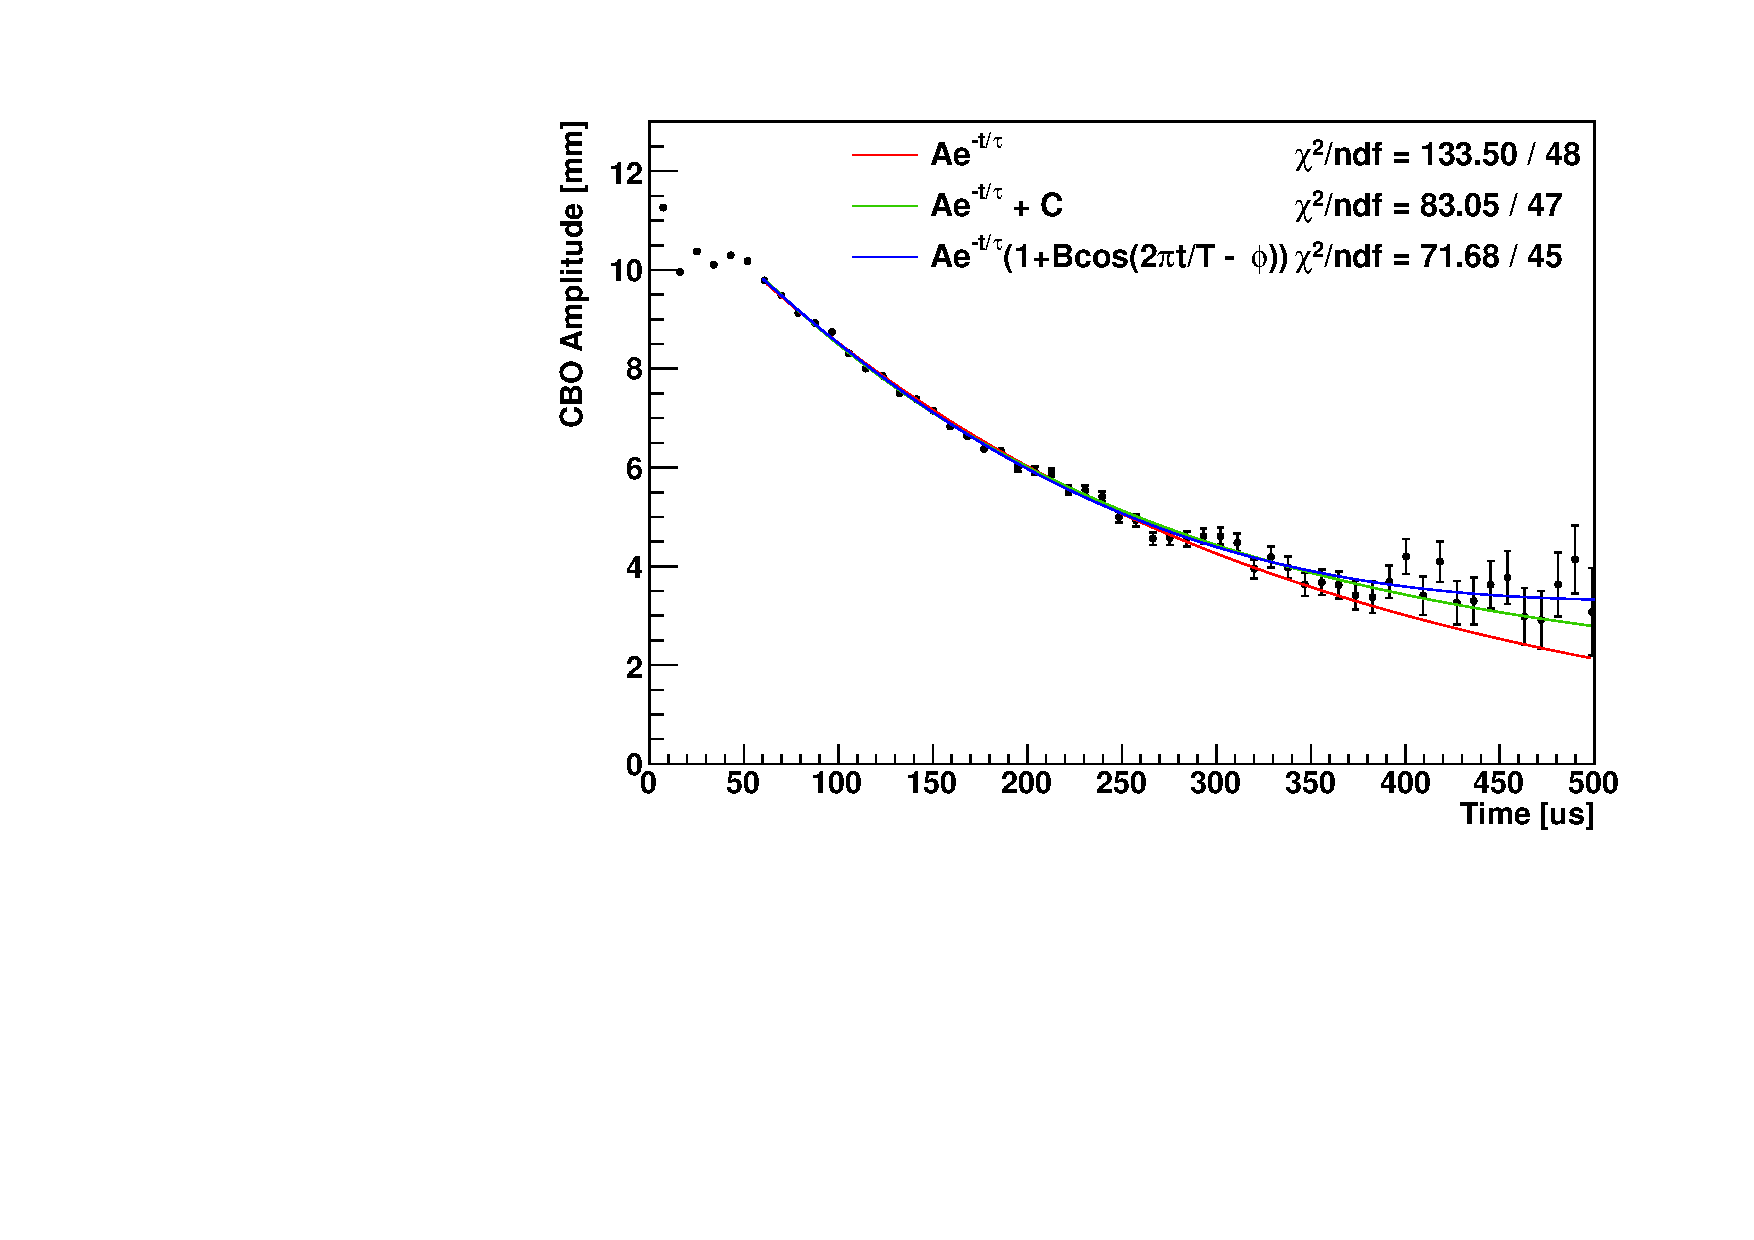
\includegraphics[width=.7\textwidth]{AmplFitOptions}
		    \caption[CBOShapeAmplitude]{Plotted is the CBO amplitude as a function of time from the tracker analysis. Three separate fit functions were used with varying degrees of success to characterize the envelope shape of the CBO (excepting the cosine modulation part). A Gaussian fit was tried with no success. The amplitude isn't fully understood at early times. The period T/$2\pi$ has a value of $\SI{114.5}{\mu s}$. Plot producd by James Mott.}
		    \label{fig:CBOShapeAmplitude}
		\end{figure}

	\subsection{CBO Lifetime}

		Because the CBO lifetime has been fixed in the fit, there is a systematic error on R. Scanning over various values of the fixed CBO lifetime allows this error to be calculated. The resulting curve of R vs the CBO lifetime turns out not to be linear, as shown in Figure \ref{fig:CBOLifetime}. Taking the uncertainty on the CBO lifetime as the error produced by the T Method fit, approximately $\SI{16}{\mu s}$, and looking at the change in R for CBO lifetime values of $180 \pm \SI{16}{\mu s}$, the systematic error on R is taken as the larger of the two at 12.1 ppb.

		\begin{figure}[]
			\centering
			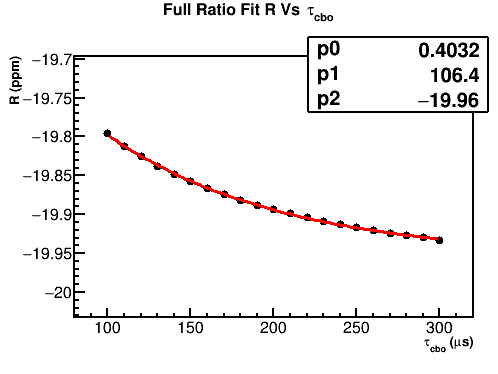
\includegraphics[width=.6\textwidth]{RatioCBO_R_Vs_tau_cbo_Canv}
		    \caption[CBOLifetime]{Plotted is the fitted R value as a function of the CBO lifetime, which has been fixed in the full ratio fit. The error bars have been removed from the plot in order to show the shape of the curve better. The points have been fitted to an exponential function which lines up nicely, $p_{0} e^{-t/p_{1}} + p_{2}$.}
		    \label{fig:CBOLifetime}
		\end{figure}





\section{Sensitivity of \texorpdfstring{$\omega_{a}$}{} to VW function}
\label{Sec:SystematicVW}

	As described in Section \ref{Sec:VW}, the vertical waist does not need to be included in the ratio fit. In order to calculate a systematic error from excluding the VW, I added the VW to the fit as described in that section, with an exponentially decaying cosine term. Since the fit is unstable in regards to the amplitude and lifetime parameters, I fixed them to values determined from a T Method fit of the same data. The results can be seen in Figure \ref{fig:VWModuloPlot}. The final fitted R value differs from the non-VW fitted function by less than 1 ppb. This is unsurprising since I'm trying to fit an effect which does not exist in the ratio.

	\begin{figure}[]
		\centering
		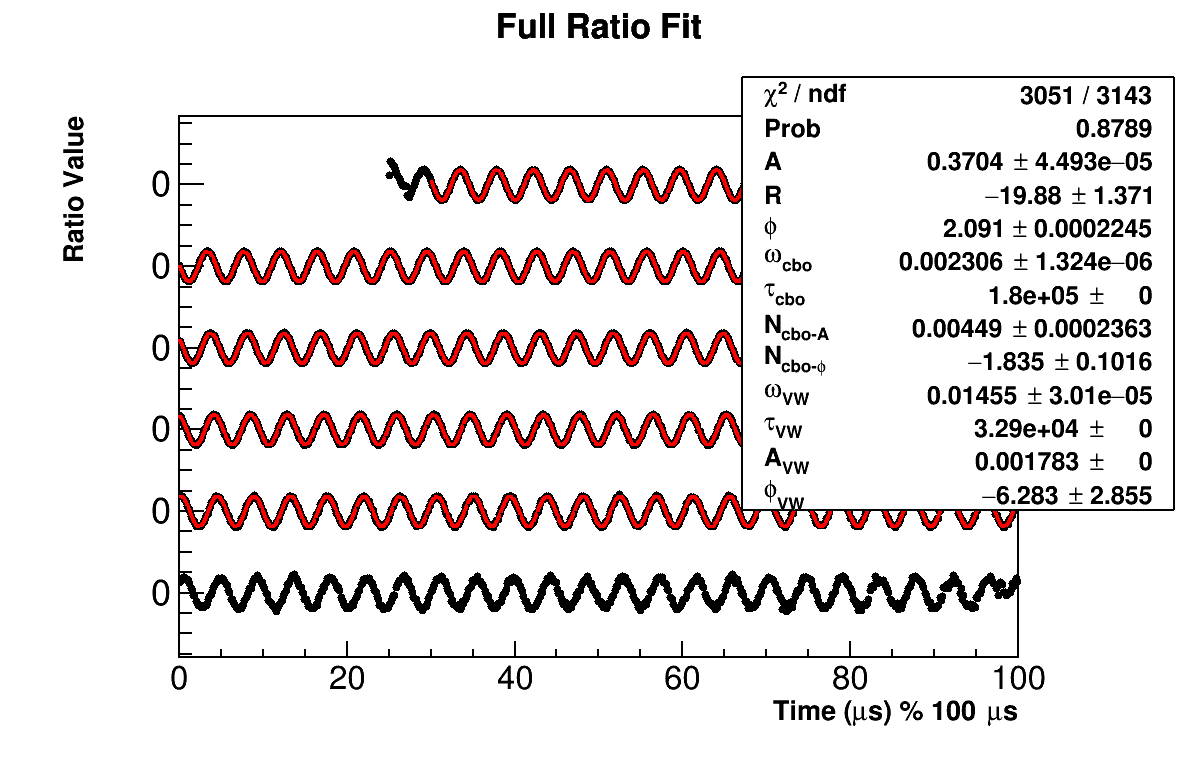
\includegraphics[width=\textwidth]{ratioCBO_moduloPlot-VW}
	    \caption[VWModuloPlot]{Fit results with the VW term included. The lifetime and amplitude of the effect have been fixed, while the frequency and phase are allowed to float. As can be seen there is a large error on the phase. The x axis is in units of $\mu$s modulo 100 $\mu$s, with successive portions of the data points and fit shifted downwards on the plot. The parameter values in the stats box for the CBO frequency and lifetime are in units of ns. R is blinded locally. The fit ranges from 30 $\mu$s to 500 $\mu$s.}
	    \label{fig:VWModuloPlot}
	\end{figure}



\section{Sensitivity of \texorpdfstring{$\omega_{a}$}{} to various effects}

	More effects to be studied - results vs bunch number, higher order beam/CBO effects, etc.

	\subsection{\gmtwo Period Guess}
	\label{SubSec:gm2Guess}

		To perform the ratio method, the \gmtwo period needs to be known a priori to high precision. By scanning over various \gmtwo period guesses the dependence of R on $T_{a}$ can be determined, as shown in Figure \ref{fig:gm2PeriodGuess}. The systematic error can then be calculated as 
			\begin{align}
				\delta R_{period} = \delta\alpha_{period} \times \frac{dR}{d\alpha_{period}}
			\end{align}
		where $\delta\alpha_{period}$ is the uncertainty on $T_{a}$. Very conservatively taking the uncertainty as 10 ppm, the systematic error on R is calcualted as $\SI{10}{ppm} \times \SI{1.62e-4}{ppm/ppm} = \SI{1.62}{ppb}$, which is completely negligible.

		\begin{figure}[]
			\centering
			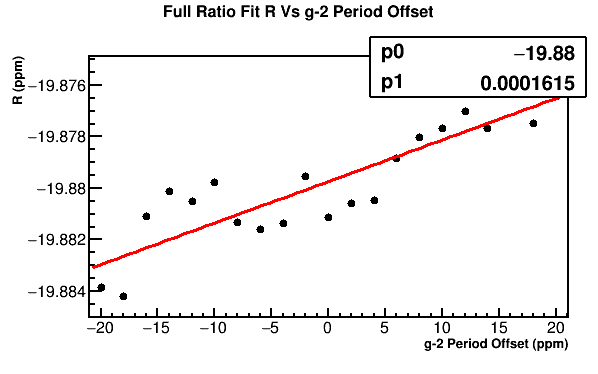
\includegraphics[width=.6\textwidth]{RatioCBO_R_Vs_gm2PeriodGuess_Canv}
		    \caption[gm2PeriodGuess]{Fitted R value as a function of the ppm level offset from the guess used for the \gmtwo period, \ref{eq:Ta}. Error bars have been removed from this plot, otherwise it appears as a flat line. The slope is .16 ppb per ppm offset in $T_{a}$.}
		    \label{fig:gm2PeriodGuess}
		\end{figure}

	\subsection{Lifetime used in weighting}
	\label{SubSec:LifetimeWeighting}

		Similarly to the \gmtwo period guesses used when constructing the time spectra for the ratio method, the lifetime of the muon is used when splitting the counts into the various histograms with different weights, as seen in Equation \ref{Eqn:Weighting}. To check for a systematic effect on R from getting this lifetime wrong, I scanned over a range of such lifetimes around the default value used, $\SI{64.4}{\mu s}$. As shown in Figure \ref{fig:weightingLifetime}, the slope is 2.632 ppb per $\mu$s. Since the uncertainty on the lifetime is much less than a microsecond, this systematic error is completely neglible.

		\begin{figure}[]
			\centering
			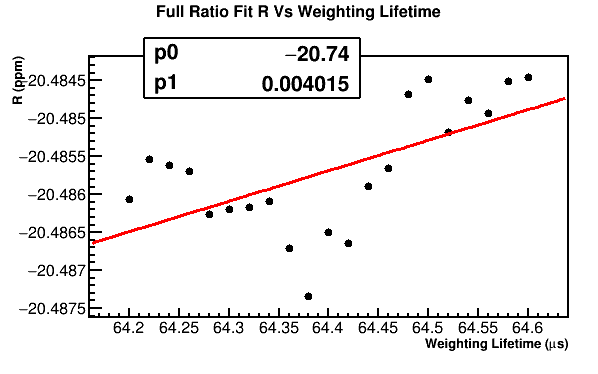
\includegraphics[width=.6\textwidth]{RatioCBO_R_Vs_weightingLifetime_Canv}
		    \caption[weightingLifetime]{Fitted R value as a function of the lifetime used in the weighting of counts into histograms. Error bars have been removed from this plot, otherwise it appears as a flat line. The slope is 2.632 ppb per $\mu$s.}
		    \label{fig:weightingLifetime}
		\end{figure}


	\subsection{Bin Width}

		The systematic uncertainty from the bin width, chosen to eliminate the fast rotation signal, was calculated by performing the histogramming and fitting stages with varying values of bin widths. The systematic uncertainty is taken as the RMS spread of the fitted R values. As shown in Figure \ref{fig:BinWidth} it is 44.5 ppb.

		\begin{figure}[]
			\centering
			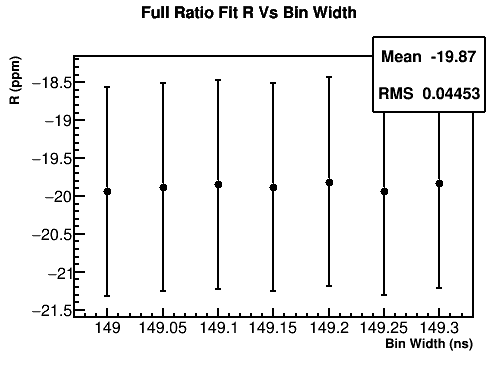
\includegraphics[width=.6\textwidth]{BinWidthComparison_R}
		    \caption[BinWidth]{Plotted are fitted R values for varying bin widths ranging from 149.00 ns to 149.30 ns in steps of 5 ns.}
		    \label{fig:BinWidth}
		\end{figure}

	\subsection{Randomization}
	\label{Sec:Randomization}

		In the histogramming phase of my analysis, random seeds are used in two places. One for the randomization of counts into the 4 separate datasets that go into the ratio, and one for the time randomization to reduce the fast rotation. It's necessary to make sure that results are consistent among random seeds, and that the final answer wasn't a particularly fortuitous or disastrous choice. In order to test this I performed fits with 20 different random seeds, the $\chi^{2}/NDF$ and fitted R values of which are plotted in Figure \ref{fig:RandomSeeds}. Results are consistent and very much within error of each other. I also performed fit start scans for a couple of the random seeds as an extra check to make sure the fitting was behaving consistently as shown in Figures \ref{fig:RandomSeedFitStartScansChi2} and \ref{fig:RandomSeedFitStartScansR}.

		\begin{figure}[]
		\centering
		    \begin{subfigure}[t]{0.45\textwidth}
			    \centering
				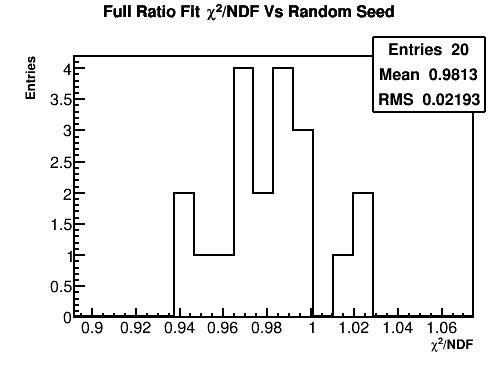
\includegraphics[width=\textwidth]{RatioCBO_Chi2NDF_Vs_Iter_Canv_hist}
			    \caption{$\chi^{2}$/NDF values for 20 random seeds.}
		    \end{subfigure}
		    \begin{subfigure}[t]{0.45\textwidth}
			    \centering
				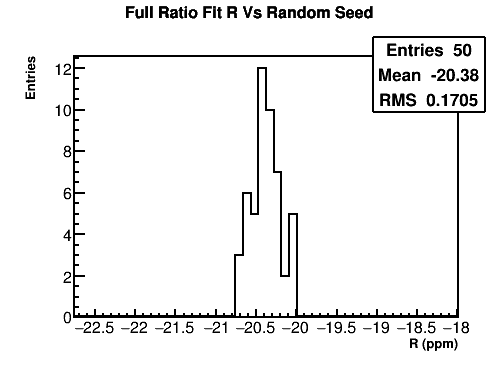
\includegraphics[width=\textwidth]{RatioCBO_R_Vs_Iter_Canv_hist}
			    \caption{R values for 20 random seeds.}
		    \end{subfigure}% %you need this % here to add spacing between subfigures
		\caption[RandomSeeds]{Plotted is the $\chi^{2}$/NDF and fitted R value for 20 random seeds.}
		\label{fig:RandomSeeds}
		\end{figure}

		\begin{figure}[]
		\centering
		    \begin{subfigure}[t]{0.45\textwidth}
			    \centering
				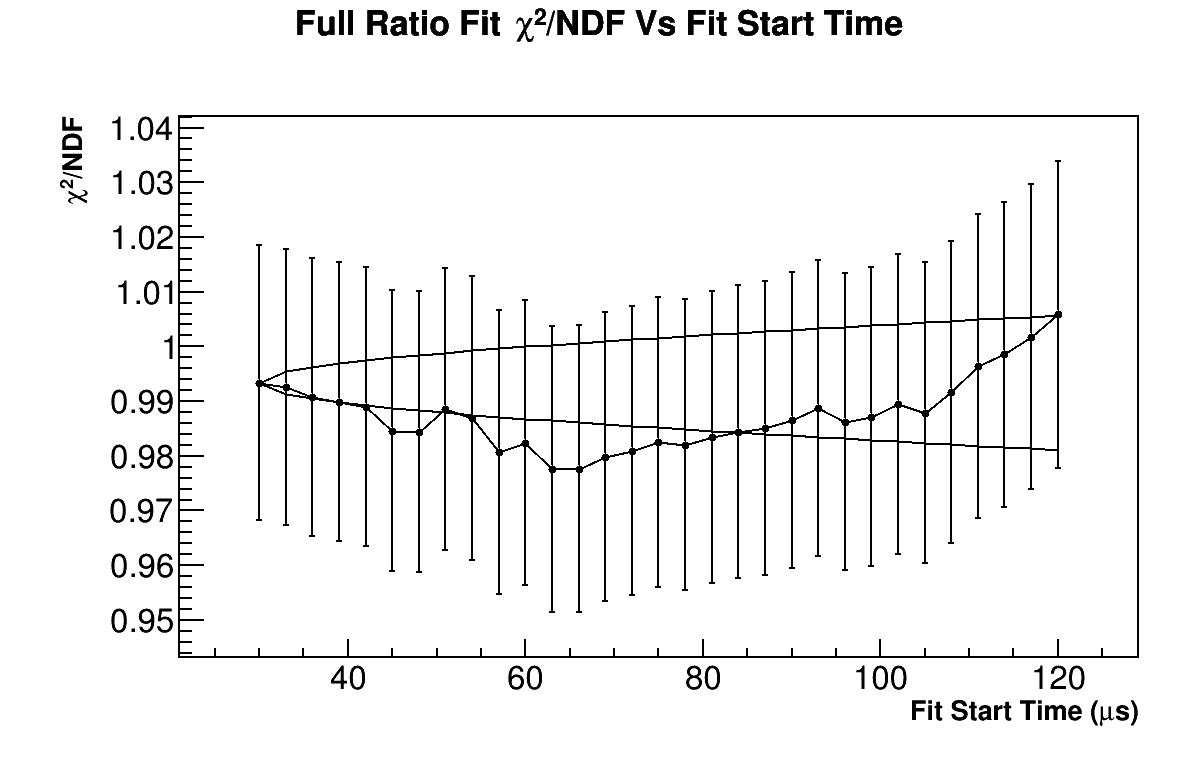
\includegraphics[width=\textwidth]{RatioCBO_Chi2NDF_Vs_FS_canv-Seed0}
			    \caption{Seed 1}
		    \end{subfigure}
		    \begin{subfigure}[t]{0.45\textwidth}
			    \centering
				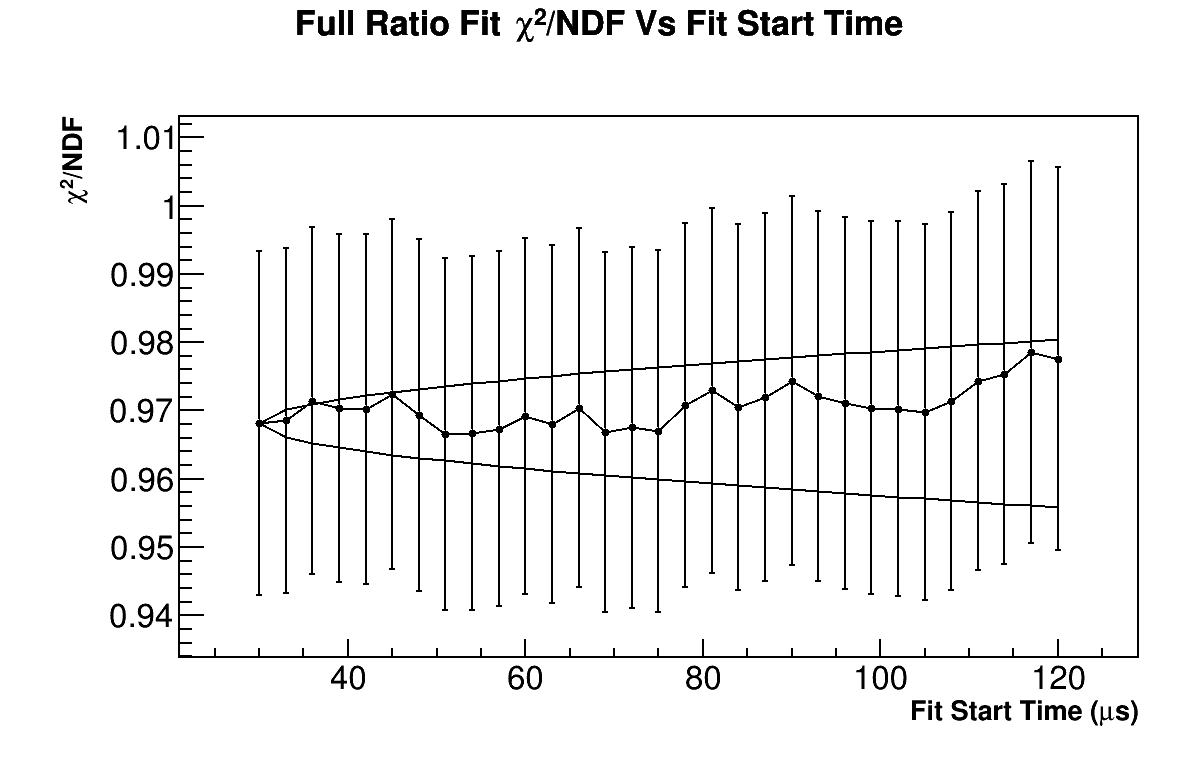
\includegraphics[width=\textwidth]{RatioCBO_Chi2NDF_Vs_FS_canv-Seed5}
			    \caption{Seed 2}
		    \end{subfigure}% %you need this % here to add spacing between subfigures
		    \vspace{4mm}
		    \begin{subfigure}[t]{0.45\textwidth}
			    \centering
				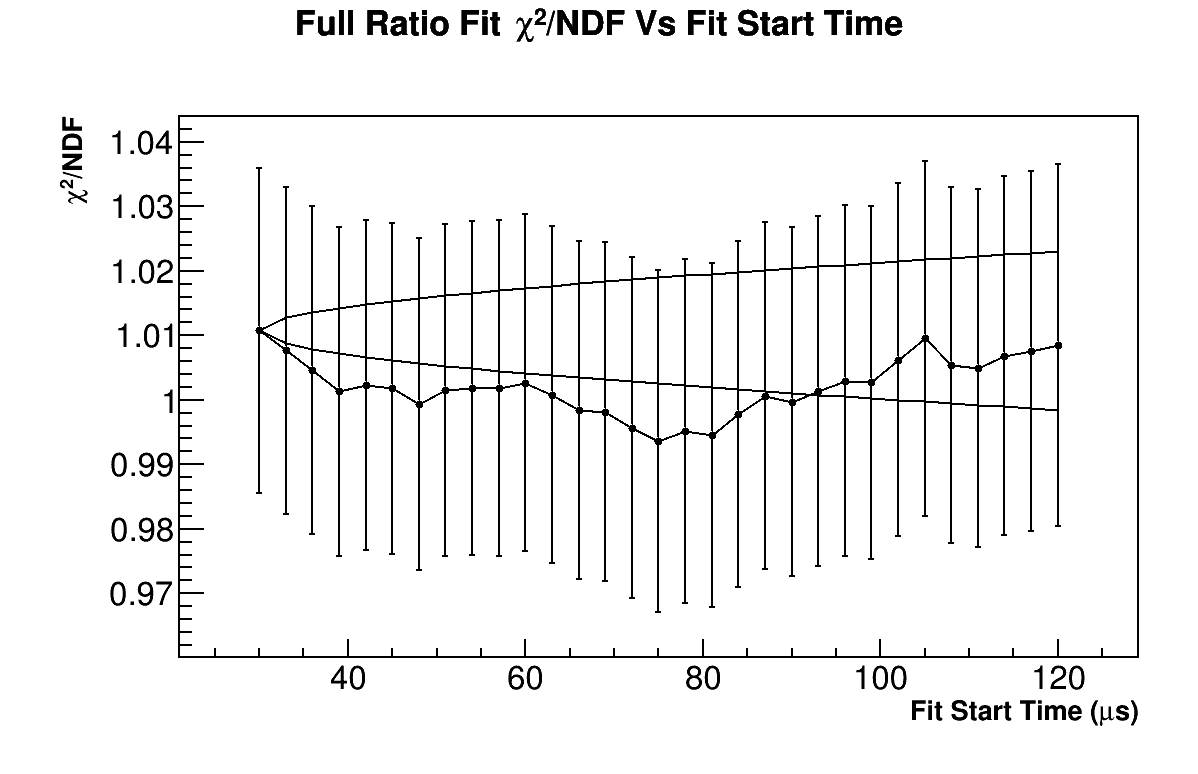
\includegraphics[width=\textwidth]{RatioCBO_Chi2NDF_Vs_FS_canv-Seed12}
			    \caption{Seed 3}
		    \end{subfigure}
		    \begin{subfigure}[t]{0.45\textwidth}
			    \centering
				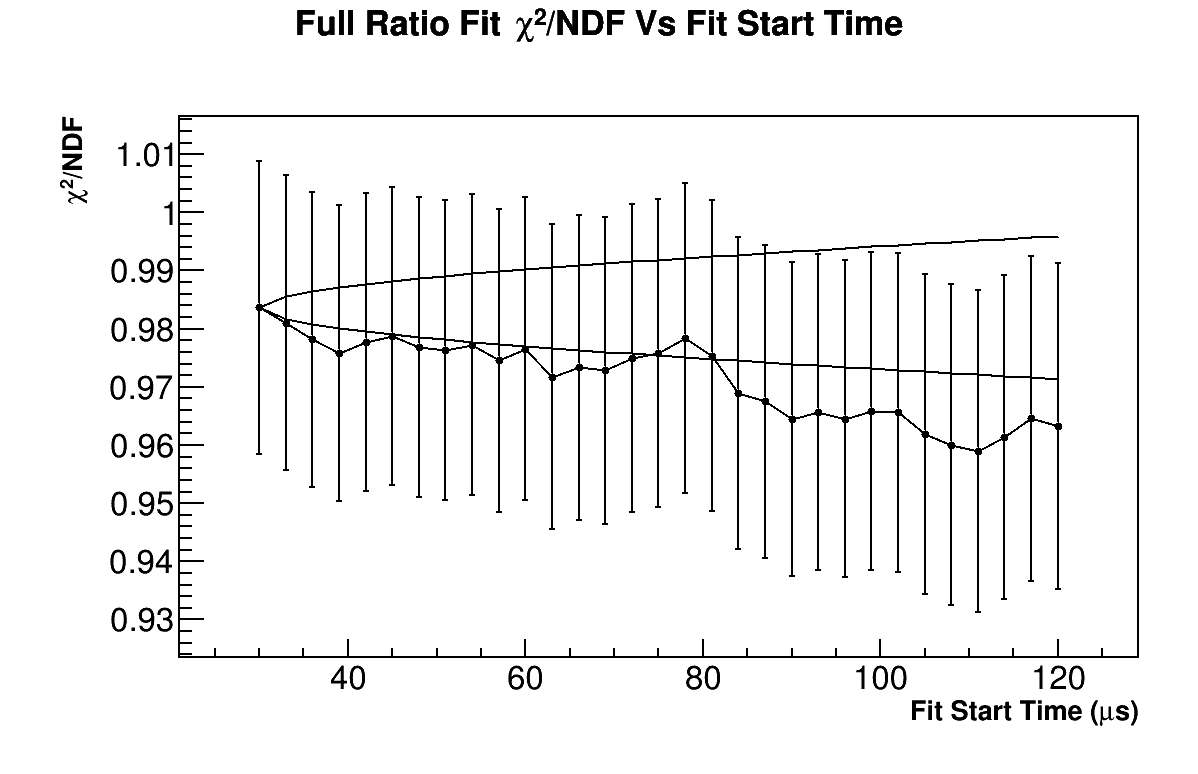
\includegraphics[width=\textwidth]{RatioCBO_Chi2NDF_Vs_FS_canv-Seed18}
			    \caption{Seed 4}
		    \end{subfigure}% %you need this % here to add spacing between subfigures
		\caption[RandomSeedFitStartScansChi2]{Fit start time scans for the \chisq for four random seeds of the randomization of the same dataset. Compare to Figure \ref{fig:RatioCBO_Chi2NDF_Vs_FS_canv}. The general behaviour of the fits vs fit start time is consistent and relatively the same, but as is seen the scans can rise and fall at different points due to the choice of randomization.}
		\label{fig:RandomSeedFitStartScansChi2}
		\end{figure}

		\begin{figure}[]
		\centering
		    \begin{subfigure}[t]{0.45\textwidth}
			    \centering
				\includegraphics[width=\textwidth]{RatioCBO_R_FS_canv-Seed0}
			    \caption{Seed 1}
		    \end{subfigure}
		    \begin{subfigure}[t]{0.45\textwidth}
			    \centering
				\includegraphics[width=\textwidth]{RatioCBO_R_FS_canv-Seed5}
			    \caption{Seed 2}
		    \end{subfigure}% %you need this % here to add spacing between subfigures
		    \vspace{4mm}
		    \begin{subfigure}[t]{0.45\textwidth}
			    \centering
				\includegraphics[width=\textwidth]{RatioCBO_R_FS_canv-Seed12}
			    \caption{Seed 3}
		    \end{subfigure}
		    \begin{subfigure}[t]{0.45\textwidth}
			    \centering
				\includegraphics[width=\textwidth]{RatioCBO_R_FS_canv-Seed18}
			    \caption{Seed 4}
		    \end{subfigure}% %you need this % here to add spacing between subfigures
		\caption[RandomSeedFitStartScansR]{Fit start time scans for the fitted R parameter for four random seeds of the randomization of the same dataset. The general behaviour of the fits vs fit start time is consistent.}
		\label{fig:RandomSeedFitStartScansR}
		\end{figure}

		I'm not so sure there should be a systematic error on R due to the randomization. Such an error should be contained within the statistical error of the final answer I believe. However I calculate one here for posterity in the manner that was done for E821,
			\begin{align}
				\delta R_{rand} = \sigma(R)/\sqrt{N-1},
			\label{Eqn:Rand}
			\end{align}
		where $\sigma(R)$ is the RMS spread in R and N is the number of random seeds fitted, in this case 20. Therefore with an RMS on R of 193.6 ppb, the systematic error on R due to the randomization is (potentially) 44.4 ppb. (The fact that simply increasing the number of seeds allows for this systematic error to reduce to zero as shown in Equation \ref{Eqn:Rand} gives greater weight to the argument that this really shouldn't be a systematic error at all, and is instead a purely statistical effect already taken care of in the fit.)


	\subsection{Bunch Number}

		I will examine R for the 8 separate bunches, once the new dataset is available.



\section{Final Systematic Uncertainty Table}


\begin{table}[H]
\centering
\setlength\tabcolsep{10pt}
\renewcommand{\arraystretch}{1.2}
\begin{tabular*}{.5\linewidth}{@{\extracolsep{\fill}}|lG|}
  \hline
  	\multicolumn{2}{|c|}{\textbf{Summary of Systematic Errors}} \\
  \hline\hline
    Systematic Error 		& \multicolumn{1}{c|}{\SI{60}{H}} \\
  \hline
	Gain(incomplete) 		&  24.8  \\
	Pileup     	     		&  37.8  \\
	Lost Muons(incomplete)  &  36.1  \\
	CBO      		 		&  38.6  \\
	VW 			     		&  \multicolumn{1}{c|}{$<1$} \\
	Bin Width        		&  44.5  \\
	Randomization    		&  44.4  \\
	Bunch Number     		&        \\
	Other   	     		&        \\
  \hline\hline		
  	Total   	     		&        \\
  \hline
\end{tabular*}
\caption{Systematic error table for the 60H dataset. All units are in ppb.}
\end{table}






